\tikzstyle{node}=[circle,inner sep=0.5mm,minimum size=5.25mm,draw = black]
\tikzstyle{bright}=[fill=black!14]
\tikzstyle{dark}=[fill=black!28]
\tikzstyle{lightEdgeStyle}=[black!20]

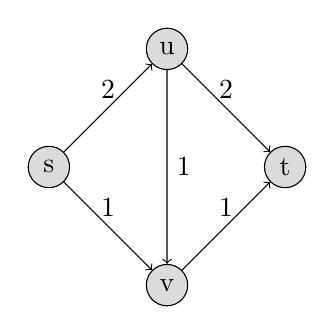
\begin{tikzpicture}[scale=1.5, bend angle = 20]

	% Obere Reihe
	\node(u) at (2,3) [node, bright] {u};
	\node(s) at (1,2) [node, bright] {s};
	\node(t) at (3,2) [node, bright] {t};
	\node(v) at (2,1) [node, bright] {v};

	\draw[->] (s) -> node[midway, above]{2} (u);
	\draw[->] (u) -> node[midway, above]{2} (t);
	\draw[->] (s) -> node[midway, above]{1} (v);
	\draw[->] (v) -> node[midway, above]{1} (t);
	\draw[->] (u) -> node[midway, right]{1} (v);
	% \foreach \i [evaluate = \i as \lastNode using \i-1] in {2,3,...,\numberOfNodes}
	% 	{
	% 		\node (Top\i) at (\i,1) [node, bright] {\i}
	% 		edge[<-] (Top\lastNode);
	% 	}


	% % Pfeile nach rechts
	% \pgfmathparse{\numberOfNodes - 2}
	% \foreach \i [evaluate = \i as \nextNode using \i+2] in {1,2,...,\pgfmathresult}
	% 	{
	% 		\foreach \j [count=\nodeIndex from \nextNode] in {\nextNode,...,\numberOfNodes}
	% 			{
	% 				\draw[->, lightEdgeStyle] (Bot\i) to [bend right] (Bot\nodeIndex);
	% 			}
	% 	}

\end{tikzpicture}
